% \documentclass[handout]{beamer}
\documentclass{beamer}

\mode<presentation>
{
  \usetheme{default}
  \usefonttheme[onlymath]{serif}
  % \usetheme{Singapore}
  % \usetheme{Warsaw}
  % \usetheme{Malmoe}
  % \useinnertheme{circles}
  % \useoutertheme{infolines}
  % \useinnertheme{rounded}

  \setbeamercovered{transparent=100}
}

\usepackage[english]{babel}
\usepackage[latin1]{inputenc}
\usepackage{textpos,alltt,listings,multirow,ulem,siunitx}
\usepackage{pdfpages}
\usepackage{multimedia}
\newcommand\hmmax{0}
\newcommand\bmmax{0}
\usepackage{bm}

% font definitions, try \usepackage{ae} instead of the following
% three lines if you don't like this look
\usepackage{mathptmx}
\usepackage[scaled=.90]{helvet}
% \usepackage{courier}
\usepackage[T1]{fontenc}
\usepackage{tikz}
\usetikzlibrary[shapes,shapes.arrows,arrows,shapes.misc,fit,positioning,trees,mindmap,backgrounds]

% \usepackage{pgfpages}
% \pgfpagesuselayout{4 on 1}[a4paper,landscape,border shrink=5mm]

\usepackage{JedMacros}

\title{User-defined Nonblocking Collectives \\ Must Make Progess}
\author{{\bf Jed Brown}}


% - Use the \inst command only if there are several affiliations.
% - Keep it simple, no one is interested in your street address.
\institute
{
  {Mathematics and Computer Science Division, Argonne National Laboratory}
}

\date{Exascale Research Conference 2012-04-16}

% This is only inserted into the PDF information catalog. Can be left
% out.
\subject{Talks}


% If you have a file called "university-logo-filename.xxx", where xxx
% is a graphic format that can be processed by latex or pdflatex,
% resp., then you can add a logo as follows:

% \pgfdeclareimage[height=0.5cm]{university-logo}{university-logo-filename}
% \logo{\pgfuseimage{university-logo}}



% Delete this, if you do not want the table of contents to pop up at
% the beginning of each subsection:
% \AtBeginSubsection[]
% {
% \begin{frame}<beamer>
%   \frametitle{Outline}
%   \tableofcontents[currentsection,currentsubsection]
% \end{frame}
% }

\AtBeginSection[]
{
  \begin{frame}<beamer>
    \frametitle{Outline}
    \tableofcontents[currentsection]
  \end{frame}
}

% If you wish to uncover everything in a step-wise fashion, uncomment
% the following command:

% \beamerdefaultoverlayspecification{<+->}

\begin{document}
\lstset{language=C}
\normalem

\begin{frame}
  \titlepage
\end{frame}

\begin{frame}{Blocking communication is the enemy}
  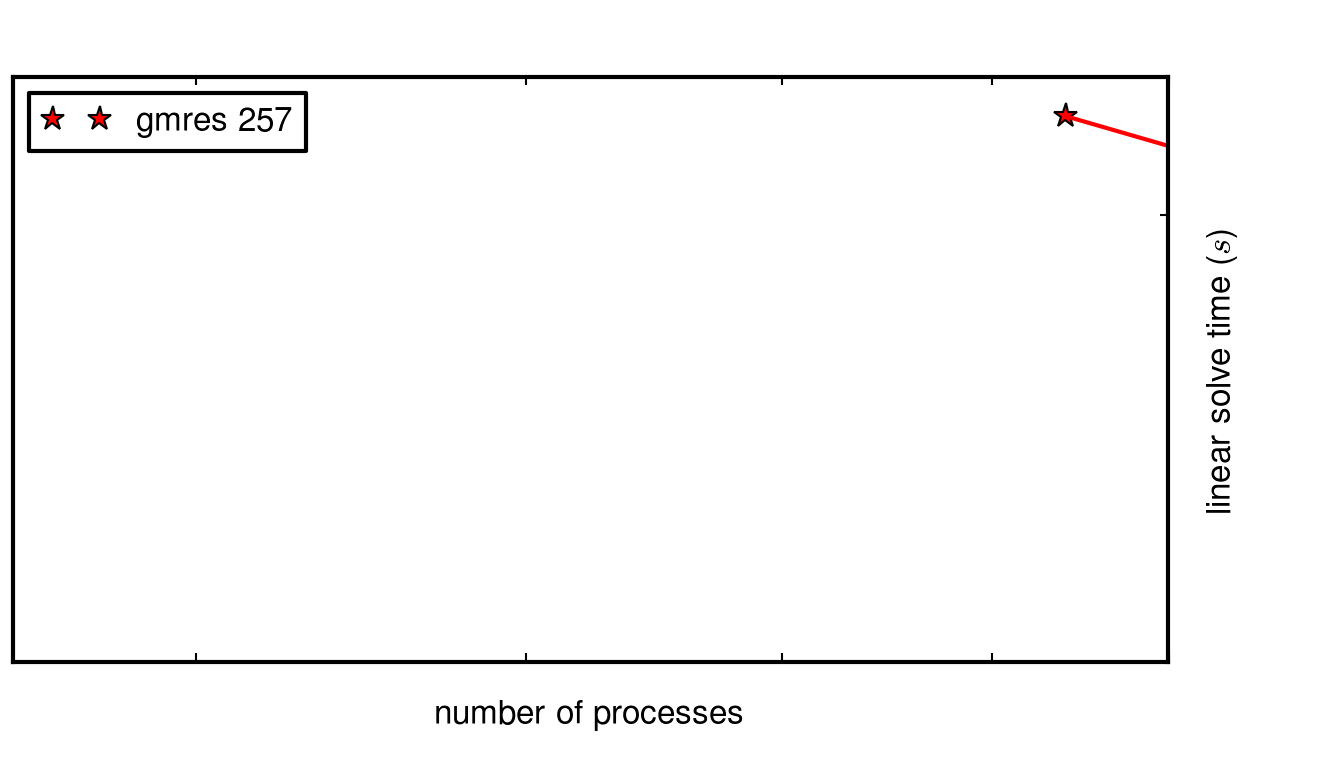
\includegraphics{figures/PipelinedGMRES} \\
  In PETSc, Block Jacobi with ILU preconditioning, {\tt -ksp\_type pgmres}
\end{frame}

\begin{frame}{Not all nonblocking algorithms belong ``upstream''}
  \begin{itemize}
  \item{\bf Tall skinny $QR$}
    \begin{itemize}
    \item Essentially {\tt Allreduce()} with side effects
    \item In this case, needed to reconstruct orthogonal $Q$.
    \end{itemize}
  \item{\bf Unstructured communication setup}
    \begin{itemize}
    \item Neighbor discovery from one-sided specification
    \item Sparse matrix assembly
    \item Many AMR applications
    \end{itemize}
  \item{\bf Fast multipole method}
    \begin{itemize}
    \item Coarse levels have little computation
    \item Can overlap with local work
    \end{itemize}
  \end{itemize}
\end{frame}

\begin{frame}{Ways to ensure progress}
  \begin{itemize}
  \item{\bf Just spawn a comm thread}
    \begin{itemize}
    \item Where should we put it?
    \item Comm threads displace computation threads and compete for shared resources.
    \item Many libraries with their own comm threads don't play nicely.
    \end{itemize}
  \item{\bf MPI Generalized Requests}
    \begin{itemize}
    \item Original MPI-2 had no way to have the request polled.
    \item Latham, Gropp, Ross, and Thakur 2007 extended added an extension for polling, but only when \emph{that request} is tested.
    \item MPI-3 nonblocking collectives are still ``special'' in that users cannot provide a nonblocking interface with comparable semantics.
    \end{itemize}
  \item{\bf Common event-driven interface}
    \begin{itemize}
    \item Could be a simple extension of MPI Generalized Requests.
    \item Any new programming models should provide something comparable.
    \end{itemize}
  \end{itemize}
\end{frame}

\end{document}
